\documentclass[11pt, oneside]{article}   	% use "amsart" instead of "article" for AMSLaTeX format
\usepackage{geometry}                		% See geometry.pdf to learn the layout options. There are lots.
\geometry{letterpaper}                   		% ... or a4paper or a5paper or ... 
%\geometry{landscape}                		% Activate for rotated page geometry
%\usepackage[parfill]{parskip}    		% Activate to begin paragraphs with an empty line rather than an indent
\usepackage{graphicx}				% Use pdf, png, jpg, or eps§ with pdflatex; use eps in DVI mode
								% TeX will automatically convert eps --> pdf in pdflatex		
\usepackage{amssymb}

%SetFonts

%SetFonts

\graphicspath{ {./images/} } 			

\title{Population Pyramids}
\author{M: 941519}
%\date{}							% Activate to display a given date or no date

\begin{document}
\maketitle


\tableofcontents
\pagebreak
\section{Cos'è una "population pyramid"}
Una "population pyramid" è una illustrazione grafica che ci permette di visualizzare la distribuzione di una popolazione (che può essere un paese in particolare, una regione del mondo, o un continente), dividendoli in bracket di anni ed in spezzandoli in segmenti in base alla proporzione tra maschi e femmine.\\

La population pyramid è formata quindi da una serie di barre ad istogramma, la popolazione è rappresentata dalla grandezza dell'asse orizzontale, ed i bracket di anni sono rappresentati dall'asse $y$.


\begin{center}
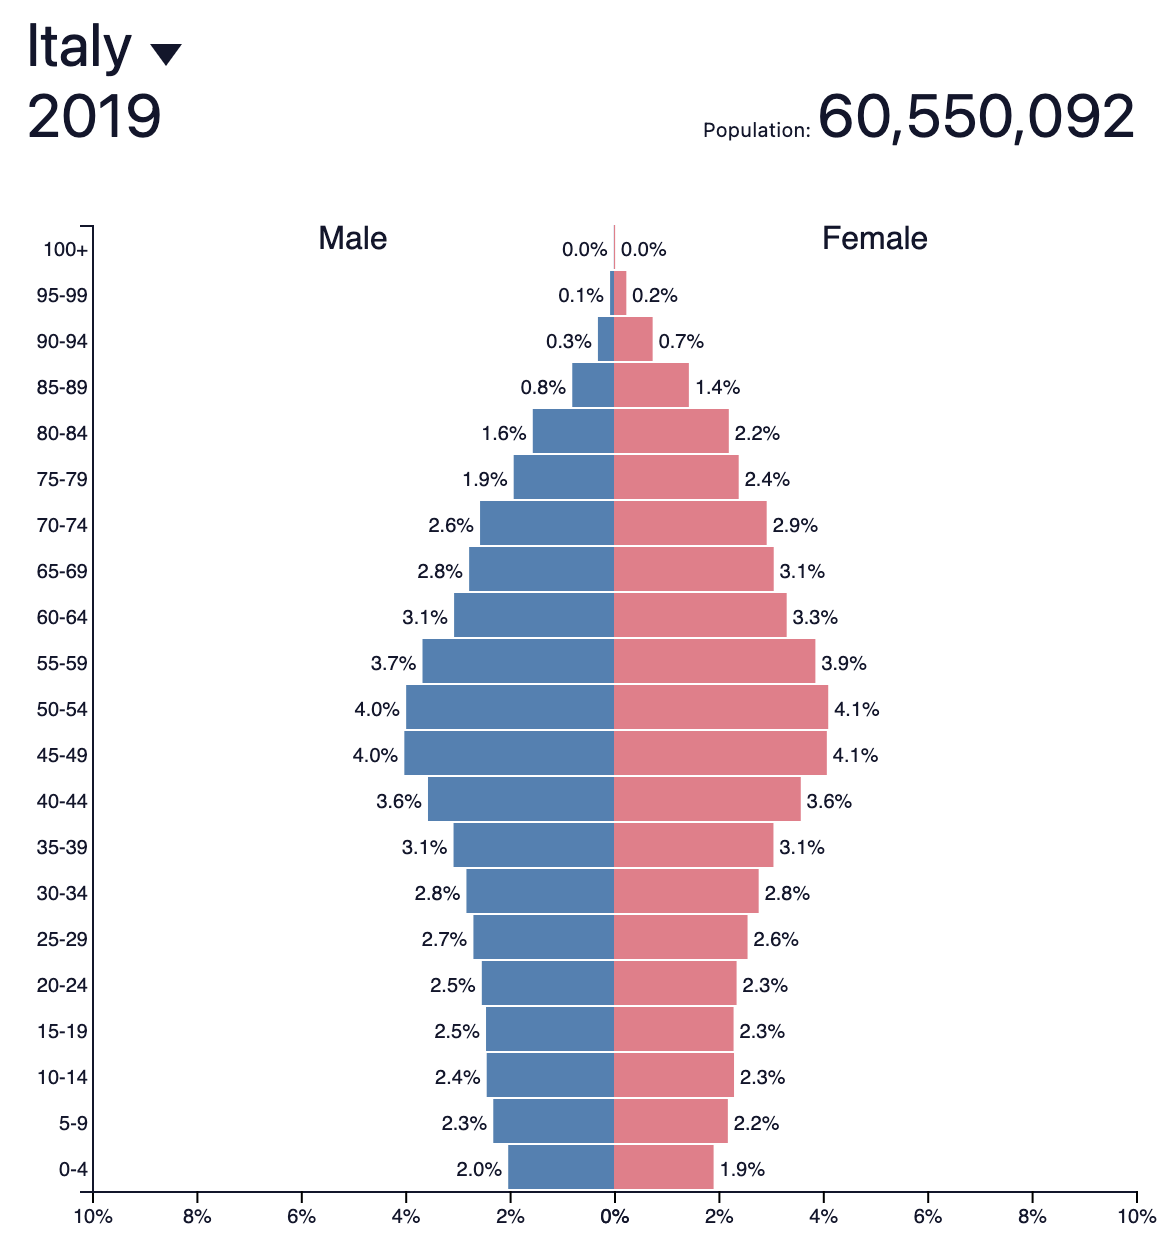
\includegraphics[scale=0.6]{pop}
\end{center}

\section{I dati necessari per costruire una "population pyramid"}
Per costruire una population pyramid abbiamo bisogno prima di tutto della popolazione totale in uno specifico anno, nel nostro esempio abbiamo preso l'Italia nell'anno 2019, e la popolazione totale è di $60.550.092$. \\
Il secondo dato fondamentale che ci serve è la proporzione, rispetto alla popolazione totale, della popolazione per ogni "age bracket". Questo dato va a rispondere alla domanda: \emph{"quante persone, maschio e femmina, vi erano, in percentuale, rispetto alla popolazione totale ?"}. Questo dato ci permette di dimensionare le varie barre del nostro grafico\\
L'ultimo dato fondamentale è la proporzione tra maschi e femmine, rispetto ad ogni "age bracket", che ci permette dimensionare, in proporzione, i maschi e le femmine.

\section{Esempio di costruzione utilizzando python}
Utilizziamo un dataset fornito da \emph{https://www.populationpyramid.net/}:
\begin{center}
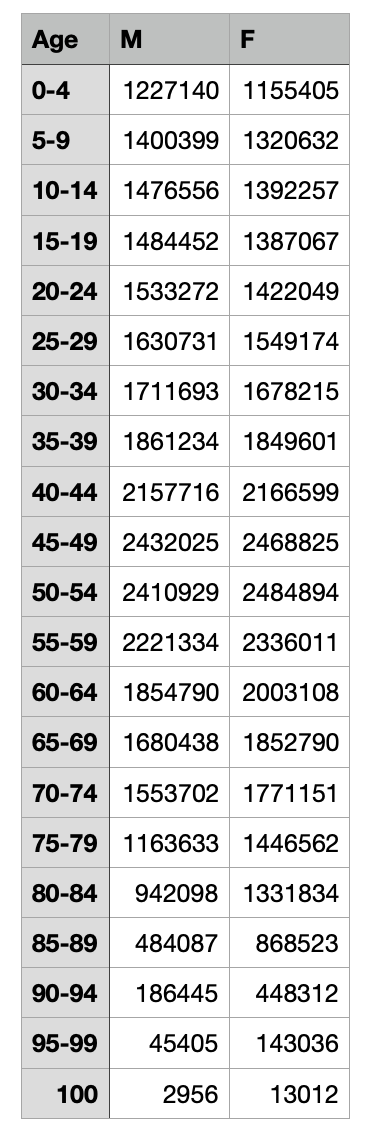
\includegraphics[scale=0.6]{popitaly}
\end{center}
Andiamo ad importare il dataset all'interno del notebook:
\begin{center}
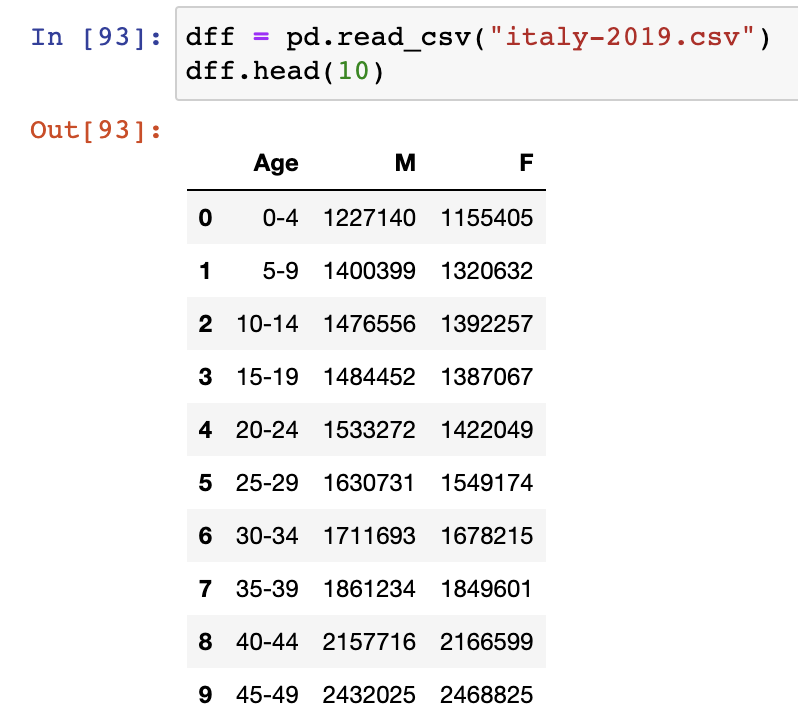
\includegraphics[scale=0.6]{popitaly2}
\end{center}
Costruiamo due liste, una per i maschi ed una per le femmine, raccogliendo i valori in base all'age bracket:
\begin{center}
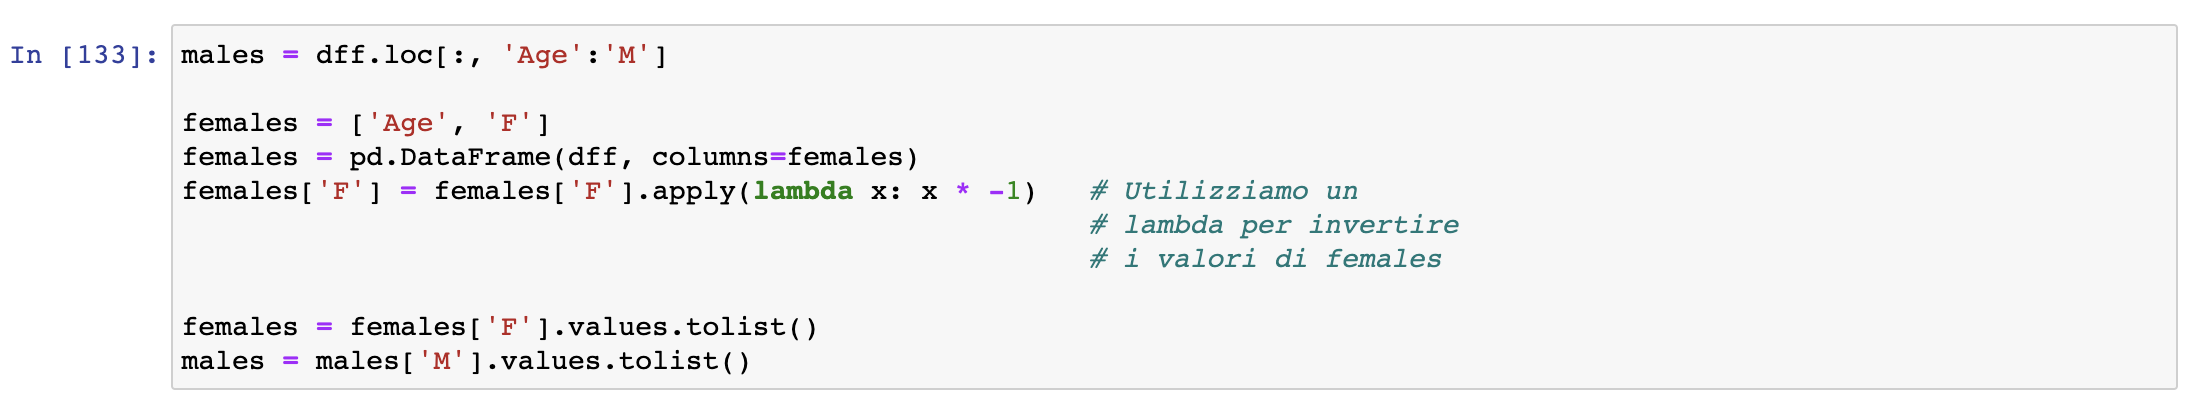
\includegraphics[scale=0.4]{popitaly3}
\end{center}
Creiamo un dataframe con headers: "Age", "Males", "Females", e utilizziamo le liste precedentemente create come input. utilizziamo quindi la libreria seaborn (basata su matplotlib) per creare la nostra population pyramid:
\begin{center}
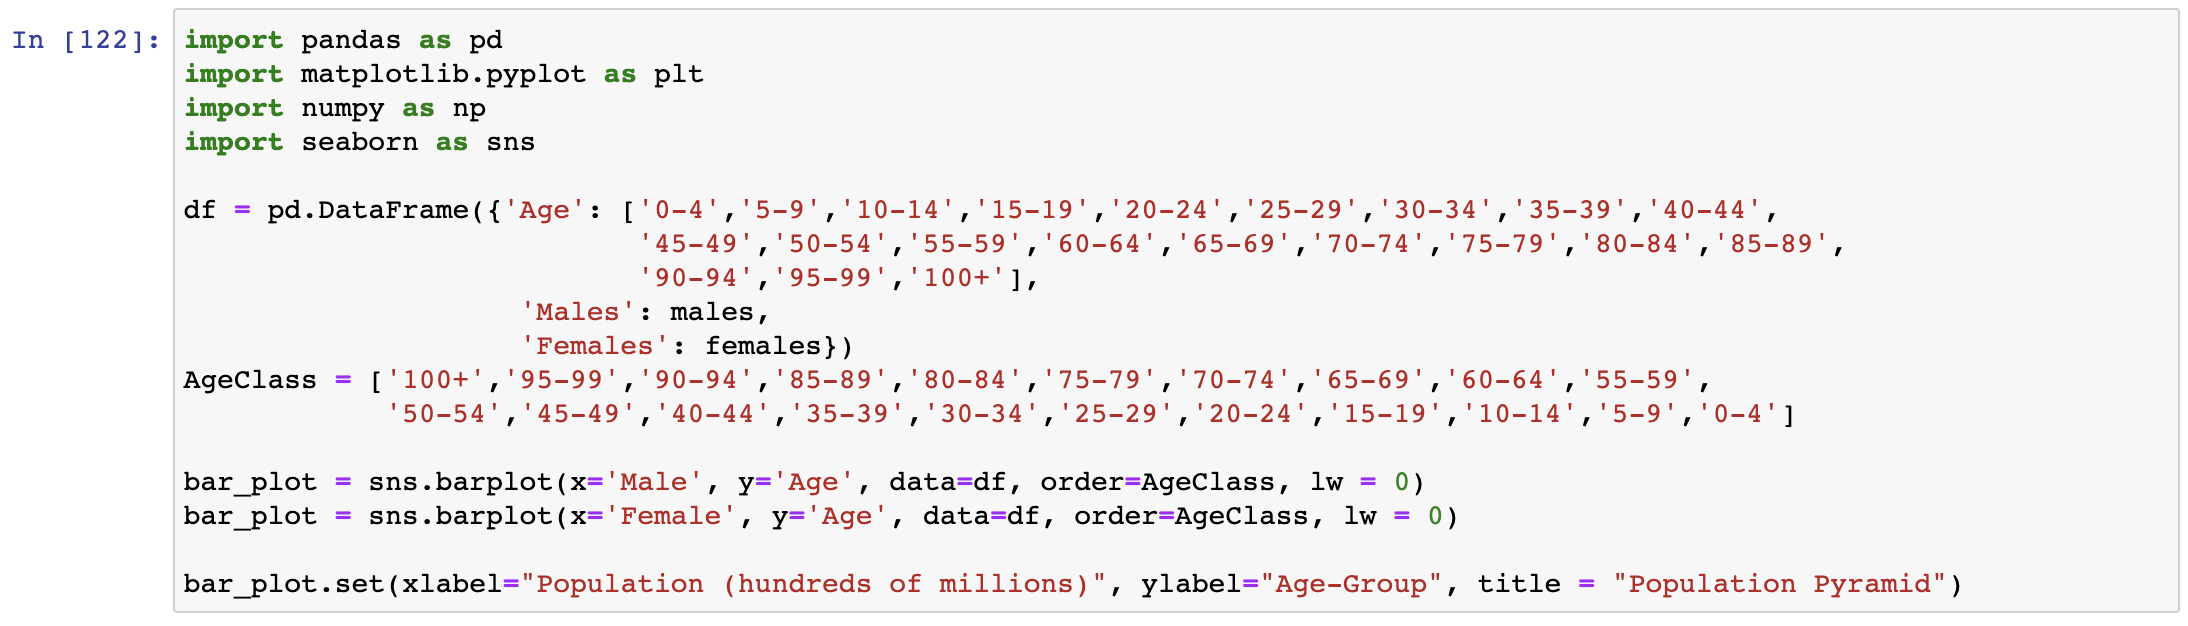
\includegraphics[scale=0.4]{popitaly4}
\end{center}
Il risultato finale è il seguente:
\begin{center}
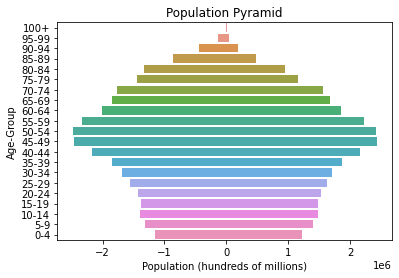
\includegraphics[scale=1]{popitaly5}
\end{center}
%\subsection{}

\section{Cosa ci dice una "population pyramid"}
\subsection{Un'appendice sull'età}
\emph{Qual'è il miglior indicatore per prevedere il comportamento di una "persona media" ed il suo contributo alla società?}\\
Ci sono molte risposte a questa domanda, il background culturale, la professione, le condizioni sociali, le norme e gli usi e costumi di un paese. L'europeo medio ad esempio risparmia di più rispetto ad un americano medio, il finanziere che gudagna 100.000\$ l'anno investe di più (anche solo perché ha più disposable income) di un meccanico che raggiunge a malapena il fine mese, e così via.\\
C'è tuttavia un dato che ci permette di prevedere, in maniera pressoché accurata, il contributo di una persona al proprio paese, l'età.

\subsubsection{Perché l'età è un indicatore così importante}
Utilizziamo la nostra "population pyramid", e consideriamo la bracket di popolazione con età superiore a 65 anni circa. Questa categoria è rappresentata solitamente dai pensionati, che hanno terminato la propria carriera lavorativa, spendono poco, investono in maniera prudente e non contribuiscono più alle casse dello stato. \\

Il secondo gruppo che ci interessa è la bracket di popolazione con età compresa tra i 30 e i 65 anni. Questo bracket di 














\end{document}  